% fundGramm.tex      pdflatex ZhCvGo15
% Diffuse globally, compute locally: a cyclist tale
% Tingnan Zhang, Daniel I. Goldman and Predrag Cvitanovi\'c

% \subsection{Grammar of fundamental domain}
% \label{s-fundGramm}

\begin{figure}[htbp]
  \begin{center}
    (a) 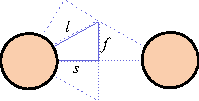
\includegraphics[width=0.35\textwidth]{diffuse7diskFundDflips}
    \\
    (b) 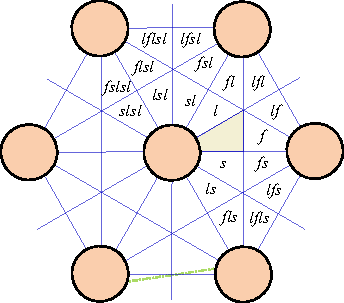
\includegraphics[width=0.35\textwidth]{diffuse7diskFundDtiles}
  \end{center}
  \caption{\label{fig-7diskFundDflips}
  (a) Three generators tile the plane by flipping the fundamental domain
  across its three strait edges. Two are elements of \Dn{6}, the
  reflection  $s$ across the short disk-disk separation, and the
  reflection $\ell$ across the long disk-disk separation. Together they
  tile the elementary cell (hexagon in \reffig{fig-schrieberFig12}\,(a)
  upper right) by copies of the fundamental domain. Translations are
  generated by the reflection $f$ that pivots a  disk center to disk
  center by a flip across the symmetry line normal to the short disk-disk
  separation.
  (b) Tiling of the 7-disk by copies of the fundamental domain, labeled
  by a (not unique) sequence of the three generators  $\{s,\ell,f\}$,
  chosen so that each sequence contain one and only on  disk-to-disk
  pivot $f$.
  }
\end{figure}
%    \TZ{2015-10-19}
%    {I do not really use the three generators to compute the fundamental
%    domain cycles, instead I use the idea of topological distinct flights
%    (\reffig{fig-fdflights}). We have yet to discuss the equivalence
%    between the 3-generators and topological distinct flight in the two
%    figures.
%    }
    \PC{2016-01-08}{Please always save the program that generated a given
    figure in \texttt{reducesymm/figSrc/} and document it in
    \texttt{reducesymm/figSrc/00ReadMe.txt}. Otherwise I have to degrade
    quality to split figures (as in \reffig{fig-fdflights}\,(c) and (b),
    and I have no way of editing labels.
    }

\begin{figure}[htbp]
  (a)\,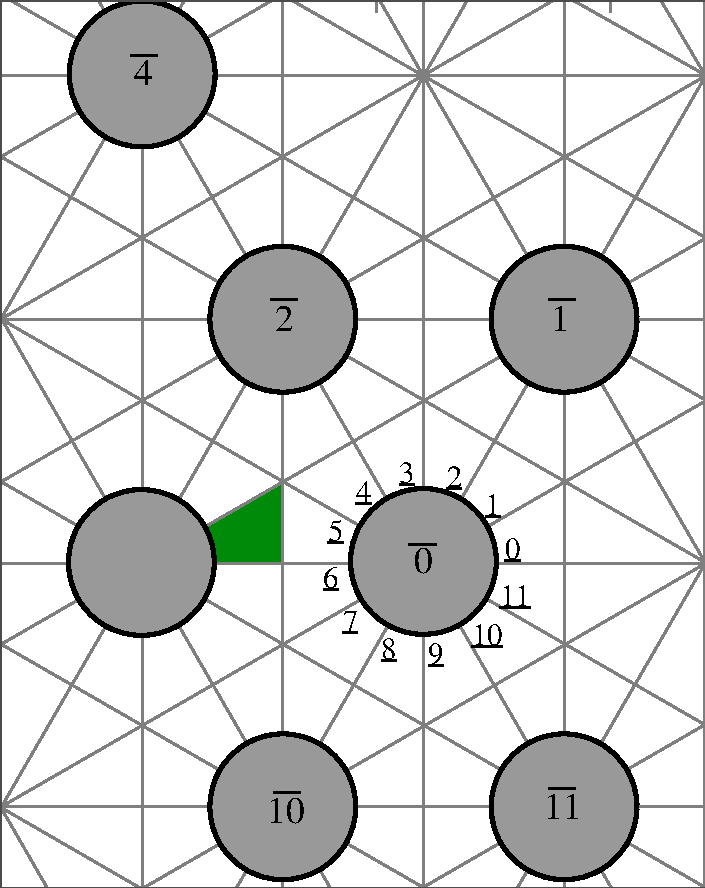
\includegraphics[width=0.35\textwidth]{diffuseFDSymbolIllustration}
  (b)\,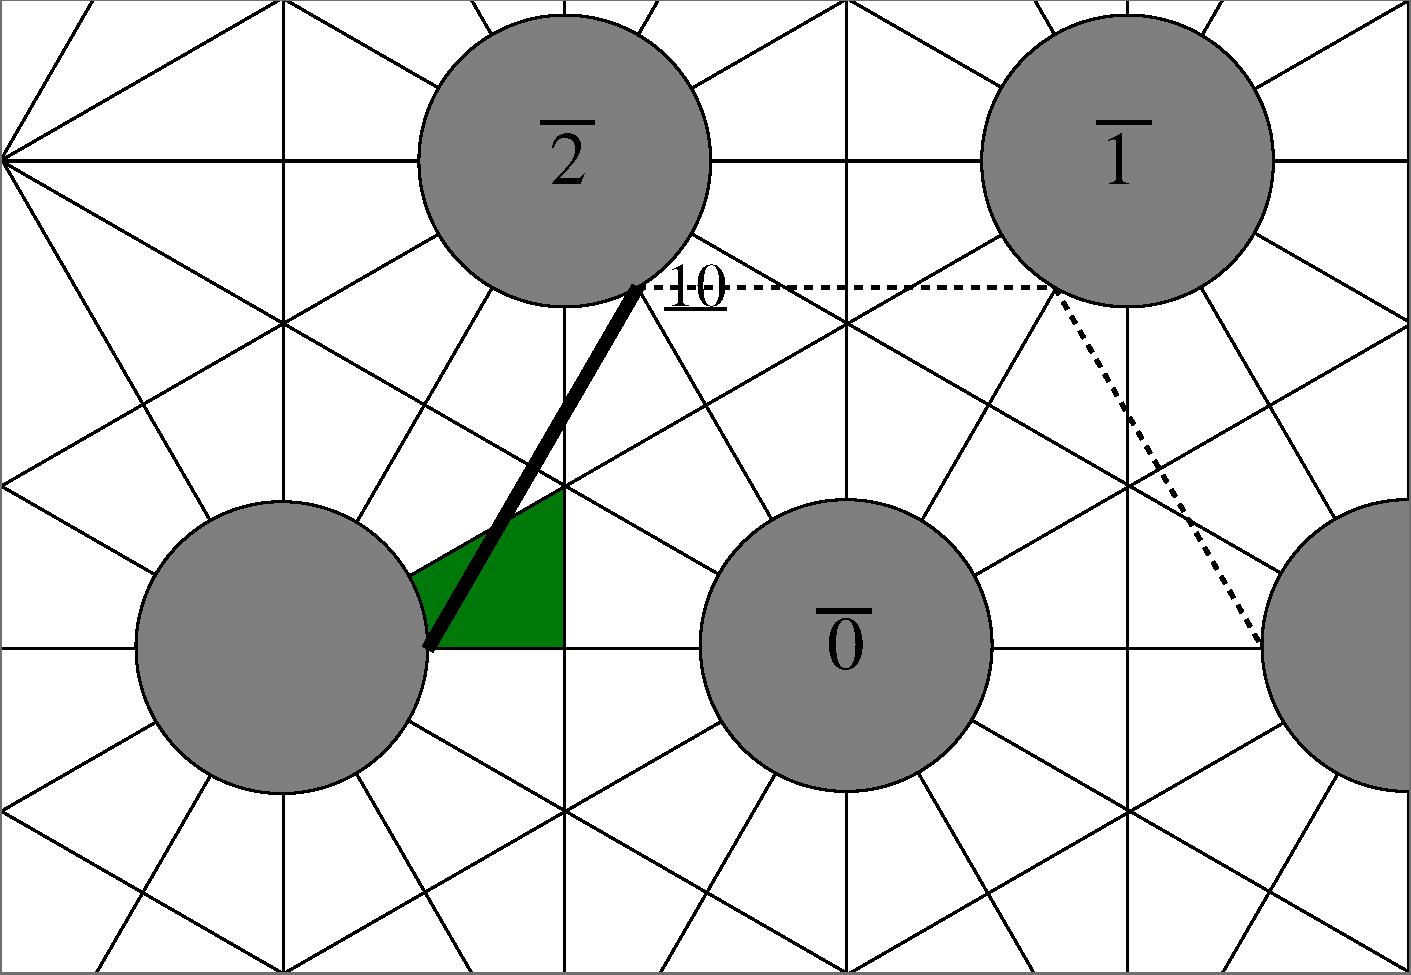
\includegraphics[width=0.35\textwidth]{diffuseFDSymbolOrbits-b}
  (c)\,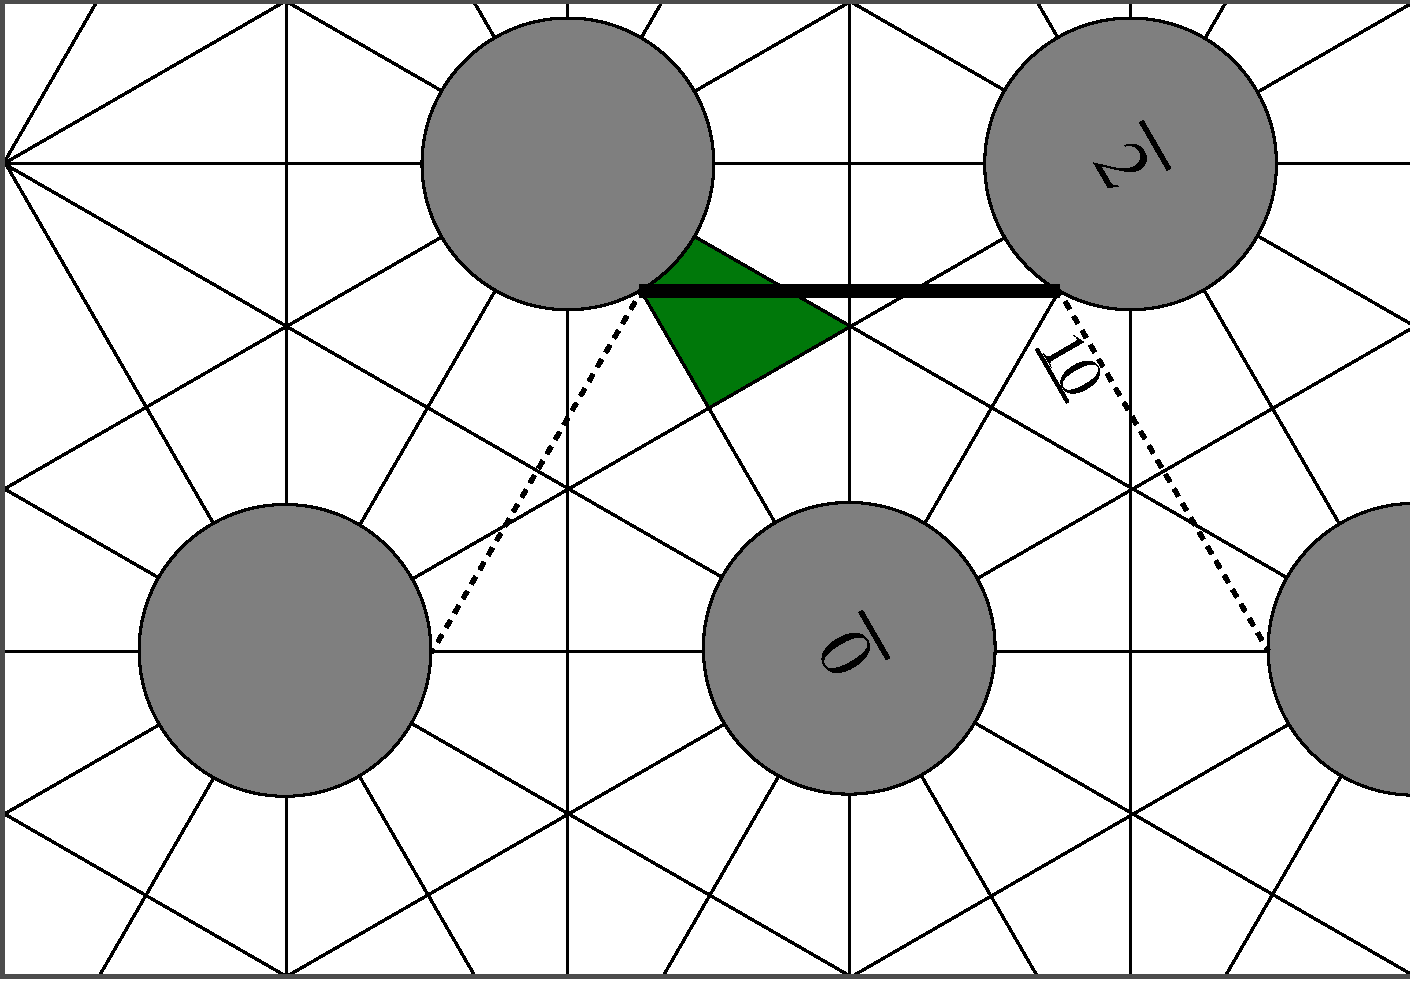
\includegraphics[width=0.35\textwidth]{diffuseFDSymbolOrbits-c}
  \caption{\label{fig-fdflights}
  Fundamental domain symbolic dynamics.
  (a) With  imposed finite horizon and starting on the edge of a disk in
  fundamental  domain (the green filled region), there are at most 6
  disks that can be reached by free flight (disks
  $\overline{0},\overline{1},\overline{2},\overline{4},\overline{10}$ and
  $\overline{11}$).
  % Similar to how elementary cell symbolic dynamics are created,
  The reflection symmetry axes partition the circumference of
  a disk into 12 segments which we
  label counterclockwise, from $\underline{0}$ to $\underline{11}$.
  (b) The fundamental domain fixed point
  $\{\overline{2},\underline{10}\}$, which corresponds to a periodic
  orbit of length 6 in elementary cell ($\cycle{0246810}$), is unwrapped
  in   global space. After each collision we re-label the disks and
  triangular   partitions according to their relative positions to the
  ``new'' fundamental   domain. In the figure labels are also rotated
  according to the point   group actions.
  }
\end{figure}

Existing elementary cell symbolic dynamics cannot generate the prime
fundamental domain orbits. While the 12 symbols partition the
elementary cell {\statesp} into distinct regions, when wrapped into
the fundamental domain {\statesp}, these regions begin to overlap.
Thus, we developed a new symbolic description to identify
the fundamental domain cycles, by means of tile generators,
which we describe next.

The symmetry of the triangular periodic Lorentz gas is the space group
$p6mm$ (see Cotton\rf{Cotton08} {\em Chemical applications of group
theory},  Chapt.~11, for a pretty discussion of the geometry of space
groups). Space group $p6mm$ has a point subgroup $C_{6v}=\Dn{6}$.
Leaving the mathematical representation of group for later discussion,
we can intuitively understand the symmetry by decomposing the
hexagonal elementary cell into 12 identical triangular tiles, as in
\reffig{fig-schrieberFig12}\,(a), upper left, the fundamental domain
and its 11 copies. The fundamental domain tiles the full hexagon, by
application of the \Dn{6} rotations around the center or reflection
along symmetry lines, \ie, the point group actions.

Tracking an arbitrary trajectory in the triangular, fundamental domain,
we can distinguish two types of bounces: those off the disk edge, and
those that in the full \statesp\ cross the symmetry axes. As discussed in
\refsect{s-FundTranslation}, the latter will add up to group operations
along the full \statesp\ trajectory.

We enumerate all the elements in the point group \Dn{6}:
\beq
\Group = \{
e, C_6^+, C_6^-, C_3^+, C_3^-, C_2,
\sigma_{d1}, \sigma_{d2}, \sigma_{d3},
\sigma_{v1},\sigma_{v2}, \sigma_{v3}
\}
\,,
\eeq
with $s=\sigma_{d}$ the reflection across the short disk-disk
separation, and $\ell=\sigma_{v}$ reflection across the long disk-disk
separation generators of \Dn{6}. The entire space group $p6mm$ is then
generated by adding a disk-to-disk generator $f$ that pivots a disk
center to another by flip across the symmetry line normal to the short
disk-disk separation, \reffig{fig-7diskFundDflips}\,(a). We find it
convenient to define $C$ as the generator of cyclic rotations by
$\pi/3$,
\beq
\ell s = C_6^- = C
\,,\quad
C^6 = e
\,;\qquad
s \ell =  C_6^+
\,,\qquad
s  =  C_6^+ \ell
\,.
\eeq
    \TZ{2015-10-22}
    {The idea is that the topological periodic orbit in the
    fundamental domain is not sensitive to the order of flips. When
    $w$ increases, one might note that a single flight along the
    orbit changes from $sf$ to $fs$. However, the relative position
    between the start and end triangular cells is always the same.}
A free flight between two disks in the full space may then be wrapped
into fundamental domain, according to the sequence of edges
$\{s,\ell,f\}$ it passed. There are many different paths when jump to
the nearest disk: it can be as simple as a single pivot $f$, or can be
more complex such like $\ell f s$ that involves crossing multiple
symmetry lines, ~\reffig{fig-7diskFundDflips}\,(b). We also note
that some symbol combinations are topologically equivalent, in the
sense that they yield the same group actions. For example, the short
jump $sf$ is topologically equivalent to $fs$, because the particle
ends up in the same copy of fundamental domain before the next
collision.

Our next task is to generate all topologically distinct itineraries from $\{s,\ell,f\}$. We can immediately realize a partial list of the equivalence relations:
\bea
f s &=& s f
\,,\nonumber\\
f \ell f&=&\ell f \ell
\,.
\eea
All longer equivalence relations in ~\reffig{fig-7diskFundDflips} can
be reduced to the above primitive ones:
\bea
f s \ell &=& s f \ell\,,\nonumber\\
\ell f\ell s &=& f \ell s f\,.
\eea

There are also some pruning rules to keep in mind. Because a free
flight cannot cross the same border twice, sequences including
$\ell\ell,ff,ss$ are forbidden. $C^3$ (and all higher orders) is also
pruned as the particle cannot cross the center hard disk; nor swirl
around it.

While the string description of flight is mathematically rigorous, it
is practically impossible to be encoded into programs for computing
the orbits, because the number of equivalent strings increases
exponentially when the length of the orbit (and also the string)
increases. However, there is a more physically intuitive way to
organize the symbols, by means of ``topological flight'',
\reffig{fig-fdflights}\,(a). In this representation, a equivalence
relation like $sf\equiv fs$ can be uniquely identified by a
combination of a disk number and a partition number
$\{\overline{0},\underline{6}\}$. Longer flight such like $\ell f \ell
s \ell f \equiv  f \ell f s \ell f \equiv f \ell s f \ell f \equiv f
\ell s \ell f \ell$ that cross many boundaries now yields a very
simple symbol pair $\{\overline{1},\underline{5}\}$.

Because this compact representation only takes into consideration the
starting and ending points of a free flight, the exponentially long
list of equivalent strings are eliminated. The topological flight
leads to a straight forward numerical scheme to find cycles. The disk
number fixes the two ends of the free flight while the partition
number limits the range of angles on the disk. Similar to searching
cycles in the elementary cell, we now have a constrained version of
convex minimization problem which can be solved using standard
non-linear optimization approach.

 \TZ{2015-11-02}
    {I have not yet talked about the pruning rule in detail here; it is
    more complicated bases on the reflection angle}
